\documentclass[11pt]{article}

\usepackage[a4paper,margin=1in]{geometry}
\usepackage[T1]{fontenc}
\usepackage{lmodern}
\usepackage{microtype}
\usepackage{textcomp}
\usepackage{graphicx}
\usepackage{array}
\usepackage{booktabs}
\usepackage{tabularx}
\usepackage{longtable}
\usepackage{enumitem}
\usepackage{xcolor}
\usepackage{float}
\usepackage{tikz}
\usepackage{hyperref}
\usetikzlibrary{arrows.meta,positioning,shapes.geometric,fit,calc}

\hypersetup{
    colorlinks=true,
    linkcolor=blue!60!black,
    urlcolor=blue!60!black,
    citecolor=blue!60!black
}

\graphicspath{{../images/}{images/}}

\setlist[itemize]{topsep=4pt,itemsep=2pt,parsep=0pt,partopsep=0pt}
\setlist[enumerate]{topsep=4pt,itemsep=2pt,parsep=0pt,partopsep=0pt}

\newcommand{\ProductName}{Dragon of North}
\newcommand{\DocTitle}{Software Requirements Specification (SRS)}
\newcommand{\DocVersion}{1.0}
\newcommand{\DocDate}{April 20, 2026}

\begin{document}
    \pagenumbering{roman}

% ---------------------------------------------------------------------------
% Title page
% ---------------------------------------------------------------------------
    \begin{titlepage}
        \centering
        {\LARGE \DocTitle \par}
        \vspace{0.8cm}
        {\Huge \ProductName \par}
        \vspace{0.8cm}
        {\Large Version \DocVersion \par}
        \vspace{0.4cm}
        {\large \DocDate \par}
        \vfill

        \begin{tabular}{@{}ll@{}}
            Prepared for: & Engineering, Security, and Operations stakeholders \\
            Prepared by:  & Project Team                                       \\
            Status:       & Submission-ready                                   \\
        \end{tabular}

        \vfill
        \begin{minipage}{0.9\textwidth}
            \small
            \textbf{Abstract.} \ProductName{} is a production-style authentication platform that provides secure identifier-based login, OTP verification, device-aware sessions, refresh-token rotation, CSRF protection, rate limiting, audit logging, and profile management. This SRS defines functional and non-functional requirements for the system, including its external interfaces, quality attributes, use cases, and diagrams.
        \end{minipage}
    \end{titlepage}

% ---------------------------------------------------------------------------
% Revision history
% ---------------------------------------------------------------------------


    \section*{Revision History}
    \begin{longtable}{@{}p{2.5cm}p{2cm}p{7.5cm}p{2.5cm}@{}}
        \toprule
        \textbf{Date} & \textbf{Version} & \textbf{Description} & \textbf{Author} \\
        \midrule
        \endhead
        \DocDate{} & \DocVersion{} & Initial version created for \ProductName{} based on an IEEE 29148-aligned structure (inspired by classic Wiegers SRS sectioning, enhanced for modern security and production operations). & Project Team \\
        \bottomrule
    \end{longtable}

    \tableofcontents
    \listoffigures
    \listoftables

    \newpage
    \pagenumbering{arabic}

% ---------------------------------------------------------------------------


    \section{Introduction}

    \subsection{Purpose}
    This document specifies the requirements for \ProductName{}, including functional behavior, external interfaces, and non-functional qualities expected of a production-grade authentication platform.

    \subsection{Scope}
    \ProductName{} provides browser-friendly authentication with cookie-based JWT transport and CSRF protection. It supports:
    \begin{itemize}
        \item Identifier-based onboarding and login (email/phone) with strong account lifecycle enforcement.
        \item Purpose-scoped OTP issuance and verification (signup/login/password reset).
        \item Device-bound sessions with refresh-token rotation and revocation.
        \item OAuth authentication using Google ID tokens (login and signup paths).
        \item User profile read/update and session visibility endpoints.
        \item Endpoint-scoped distributed rate limiting and security observability (metrics/audit).
    \end{itemize}

    Out of scope for this SRS: multi-factor authentication beyond OTP (e.g., WebAuthn), full RBAC administration UI, and enterprise identity providers beyond Google.

    \subsection{Definitions, Acronyms, and Abbreviations}
    \begin{tabularx}{\textwidth}{@{}lX@{}}
\toprule
\textbf{Term} & \textbf{Meaning} \\
\midrule
API & Application Programming Interface (HTTP/JSON in this system). \\
CSRF & Cross-Site Request Forgery; mitigated using a cookie + header echo token strategy. \\
JWT & JSON Web Token; used for access and refresh tokens, signed with RSA keys. \\
OTP & One-Time Password; short-lived verification code for purpose-scoped flows. \\
RBAC & Role-Based Access Control; data model support exists for future expansion. \\
SLO & Service Level Objective; reliability/latency targets for production operations. \\
\bottomrule
    \end{tabularx}

    \subsection{References}
    Key internal references (project documentation):
    \begin{itemize}
        \item \texttt{docs/system/system-overview.md}
        \item \texttt{docs/system/security.md}
        \item \texttt{docs/contracts/api.md}
        \item \texttt{docs/features/} feature notes
        \item \texttt{docs/decisions/} architecture decision records
    \end{itemize}

    \subsection{Document Overview}
    This document is organized as follows: \emph{Overall Description} describes system context and constraints; \emph{External Interface Requirements} defines interface requirements; \emph{System Features} specifies system features and functional requirements; \emph{Non-functional Requirements} defines non-functional requirements; \emph{Use Cases} includes representative use cases; and \emph{Diagrams} provides diagrams for context, architecture, and flows.

% ---------------------------------------------------------------------------


    \section{Overall Description}\label{sec:overall}

    \subsection{Product Perspective}
    \ProductName{} is a backend-centric authentication platform with an optional web frontend for user interaction. The backend exposes a REST API over HTTPS and persists data in PostgreSQL. Redis is used for distributed rate limiting. External integrations include AWS (SES/SNS) for OTP delivery, Google OAuth token verification, and a media provider for avatar hosting.

    \subsection{Product Functions}
    At a high level, the system:
    \begin{itemize}
        \item Determines account status for a provided identifier (email/phone).
        \item Performs sign-up and login using local credentials and/or OAuth.
        \item Issues, verifies, and consumes OTP codes for purpose-scoped flows.
        \item Mints access/refresh JWTs, sets cookies, rotates refresh tokens, and revokes sessions.
        \item Enforces CSRF protection for state-changing requests.
        \item Applies endpoint-scoped rate limiting before authentication processing.
        \item Provides profile and session management endpoints for authenticated users.
        \item Records audit events and emits operational metrics.
    \end{itemize}

    \subsection{User Classes and Characteristics}
    \begin{tabularx}{\textwidth}{@{}lX@{}}
\toprule
\textbf{User Class} & \textbf{Description} \\
\midrule
End user & Uses browser UI or client app to sign up, log in, manage profile, and control sessions. \\
Client developer & Integrates applications with the API contracts, cookies, CSRF, and error envelope conventions. \\
Operations/SRE & Deploys and monitors the system (PostgreSQL, Redis, backend services), manages keys and configuration. \\
Security reviewer & Validates security properties (token lifecycle, CSRF, rate limiting, audit). \\
\bottomrule
    \end{tabularx}

    \subsection{Operating Environment}
    \begin{itemize}
        \item Backend: Java 21, Spring Boot, Spring Security, JPA/Hibernate.
        \item Data store: PostgreSQL 16 with Flyway migrations.
        \item Cache/infra: Redis 7 for rate limiting (Bucket4j).
        \item Deployment: Docker-based (containerized services), CI/CD automated on main branch.
        \item Client: Modern web browsers; optional frontend application.
    \end{itemize}

    \subsection{Design and Implementation Constraints}
    \begin{itemize}
        \item Cookie-based token transport (HttpOnly) requires a CSRF strategy for mutating requests.
        \item Refresh tokens must be rotated and validated against persisted session state; raw refresh tokens must never be stored.
        \item Rate limiting must run before authentication filters to reduce attack surface load.
        \item Cryptographic keys (RSA) must be provided securely and rotated via operational process.
        \item JSON payloads use \texttt{snake\_case} and a consistent response envelope.
    \end{itemize}

    \subsection{User Documentation}
    \begin{itemize}
        \item API documentation via Swagger UI (runtime deployment).
        \item Project overview in \texttt{README.md}.
        \item Detailed system notes and contracts under \texttt{docs/}.
    \end{itemize}

    \subsection{Assumptions and Dependencies}
    \begin{itemize}
        \item Access to external providers (AWS SES/SNS, Google token verification) is available in production environments.
        \item Clients can store and send cookies and CSRF headers correctly (same-site and secure attributes configured by environment).
        \item Time synchronization and reliable randomness are available for OTP generation and token expiry semantics.
        \item Redis availability impacts rate limiting accuracy and behavior; PostgreSQL availability impacts login/refresh operations.
    \end{itemize}

% ---------------------------------------------------------------------------


    \section{External Interface Requirements}\label{sec:external}

    \subsection{User Interfaces}
    The system may be deployed with a web user interface. The UI requirements focus on clarity, safety, and session visibility.

    \begin{figure}[H]
        \centering
        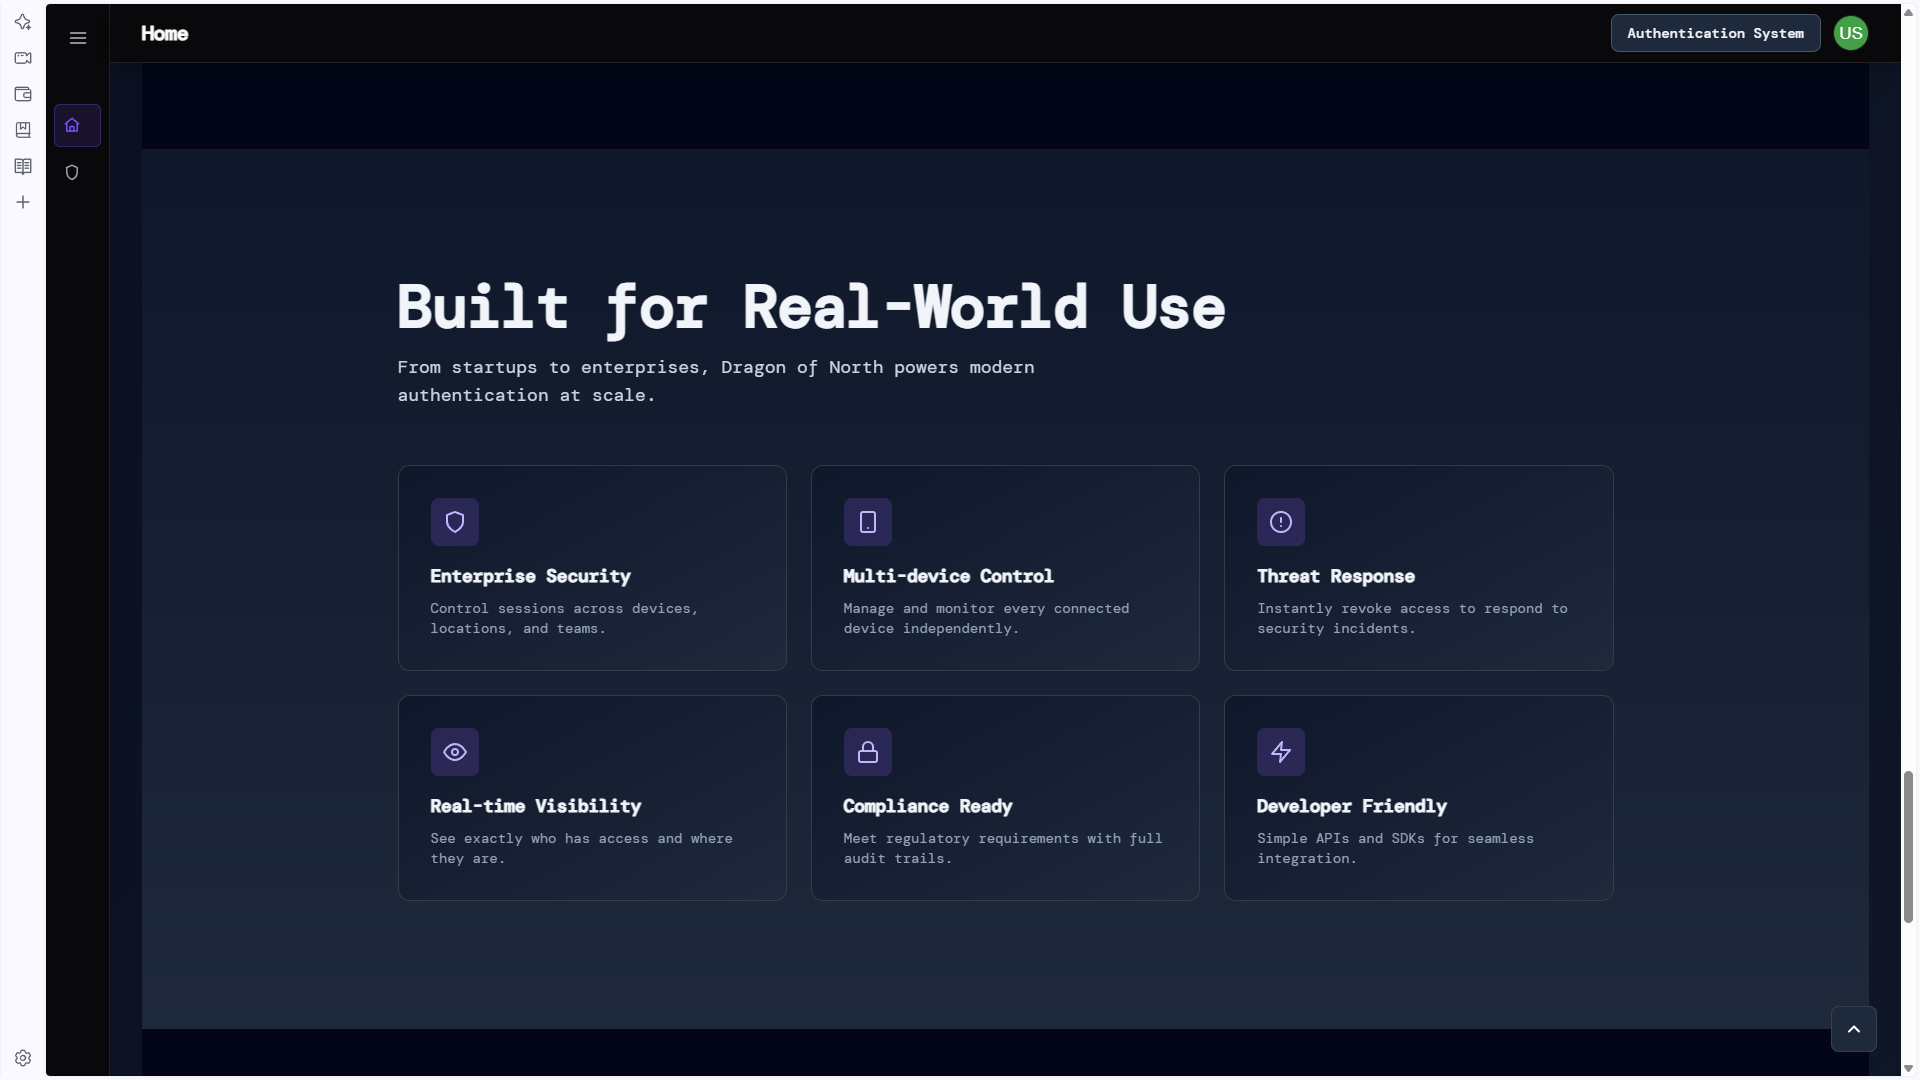
\includegraphics[width=0.95\linewidth]{img_5.png}
        \caption{Landing page concept highlighting real-world use positioning (illustrative).}
        \label{fig:ui-landing}
    \end{figure}

    \begin{figure}[H]
        \centering
        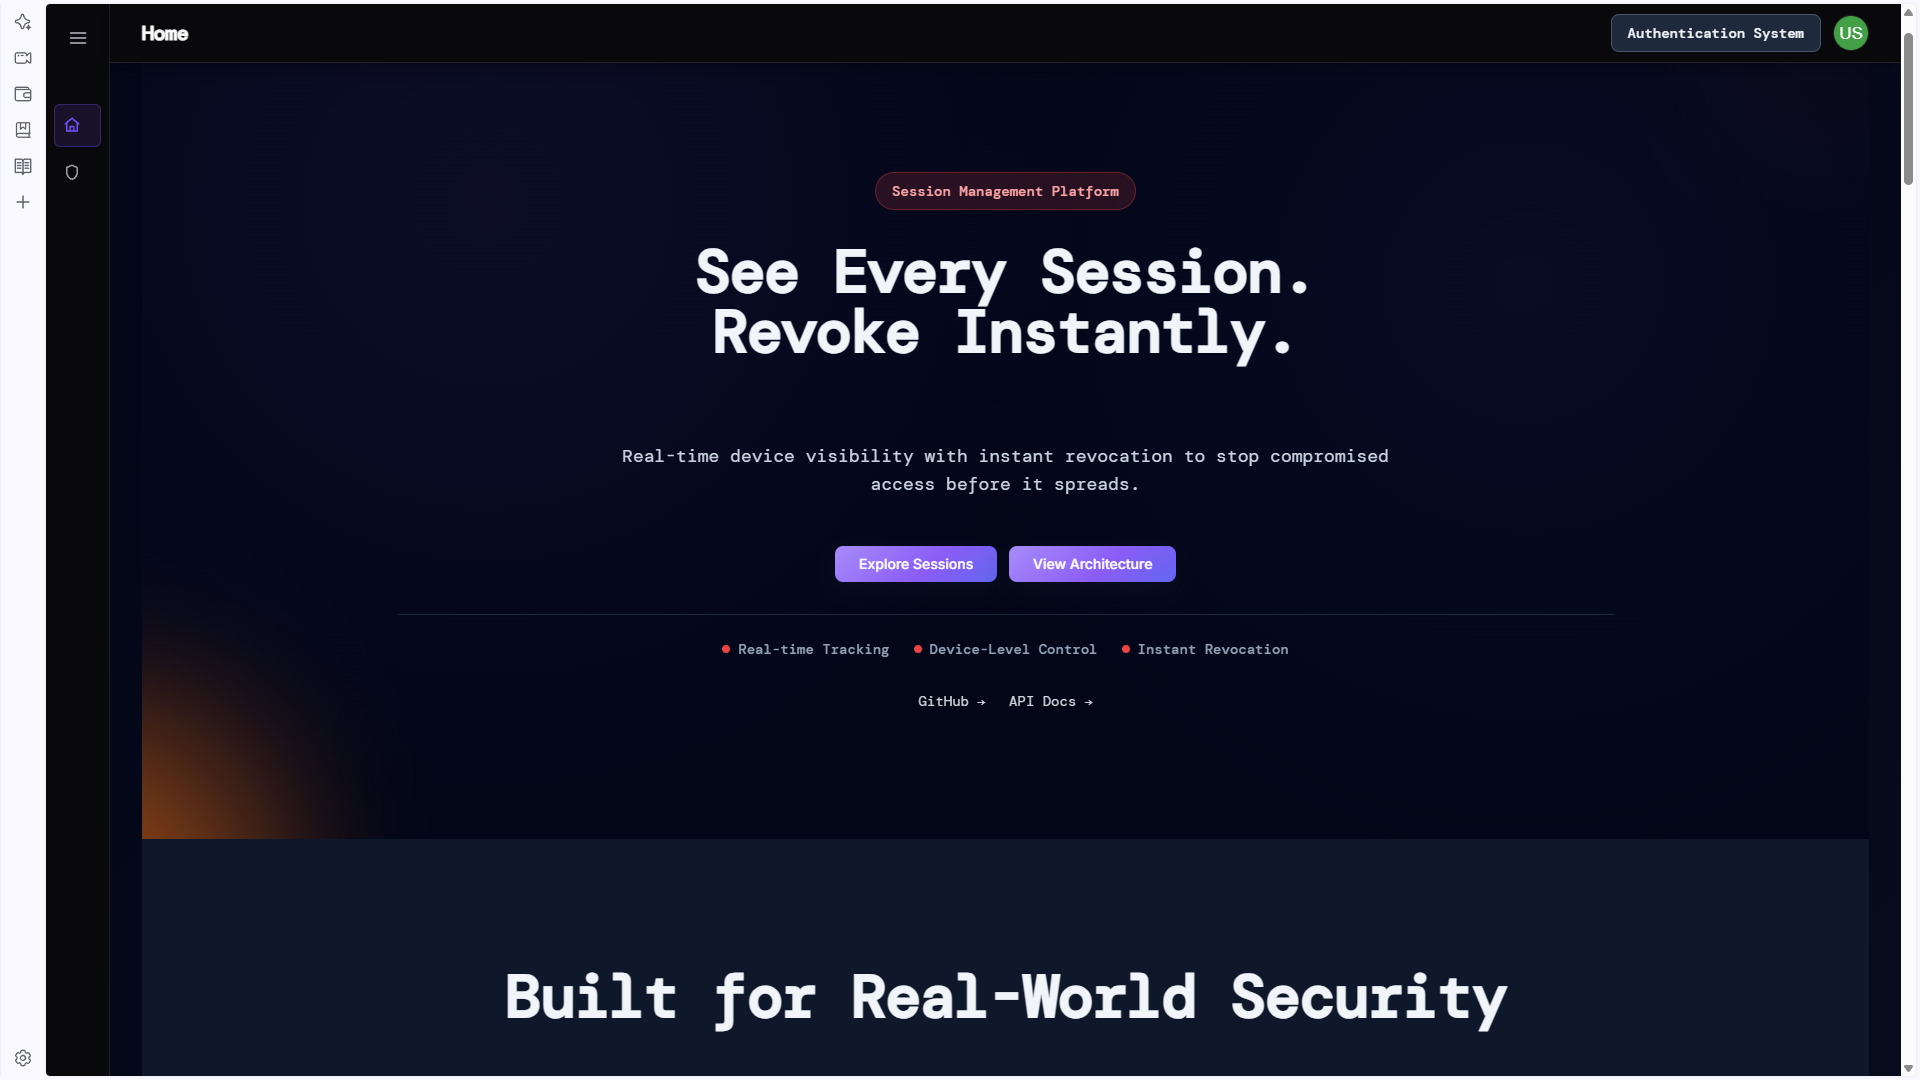
\includegraphics[width=0.95\linewidth]{img_6.png}
        \caption{Session management positioning emphasizing visibility and instant revocation (illustrative).}
        \label{fig:ui-sessions}
    \end{figure}

    \begin{figure}[H]
        \centering
        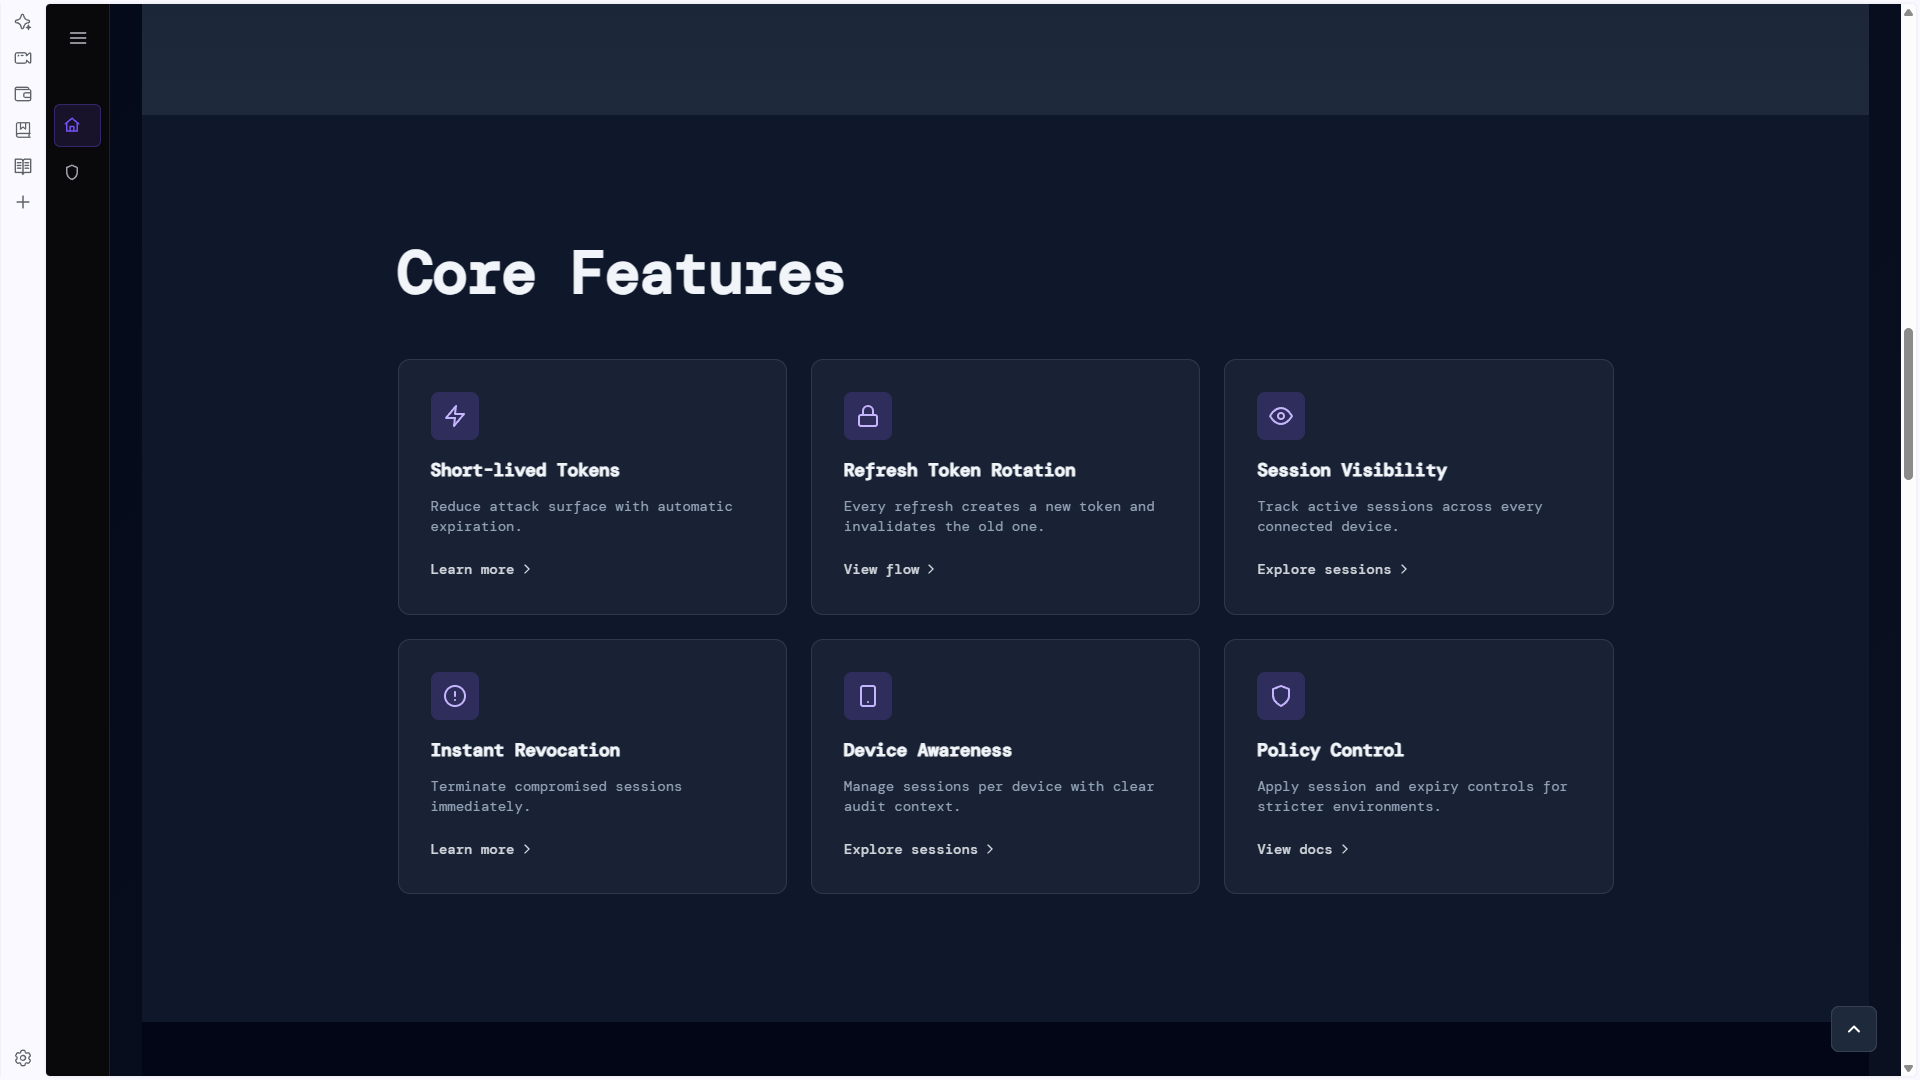
\includegraphics[width=0.95\linewidth]{img_7.png}
        \caption{Core feature messaging for token/session control (illustrative).}
        \label{fig:ui-features}
    \end{figure}

    \textbf{UI requirements:}
    \begin{itemize}
        \item UI-1: Provide a sign-up and login experience that clearly communicates the authentication stage (identify \textrightarrow{} create account \textrightarrow{} verify OTP \textrightarrow{} login).
        \item UI-2: Provide session visibility and revocation UX so users can detect and respond to suspicious activity.
        \item UI-3: Prevent accidental unsafe actions (e.g., clear confirmation for ``revoke other devices'', ``delete account'').
        \item UI-4: Avoid exposing sensitive tokens to JavaScript (no localStorage tokens; rely on cookies).
    \end{itemize}

    \subsection{Software Interfaces}
    \textbf{Backend API (HTTP/JSON).}
    \begin{itemize}
        \item SI-1: REST endpoints must conform to \texttt{application/json} and a standard response envelope:
        \texttt{\detokenize{{"status":"success|failed","message":"...","data":...}}}.
        \item SI-2: JSON field naming must use \texttt{snake\_case}.
        \item SI-3: Authentication relies on \texttt{access\_token} and \texttt{refresh\_token} cookies; clients must support cookie handling.
        \item SI-4: Mutating endpoints must require CSRF header \texttt{X-XSRF-TOKEN} except for explicitly documented bypass endpoints.
        \item SI-4.1: The system shall provide a CSRF bootstrap endpoint that sets a CSRF cookie and returns the token in the response body for client initialization.
    \end{itemize}

    \textbf{Data store (PostgreSQL).}
    \begin{itemize}
        \item SI-5: Persist users, providers, sessions, OTP tokens, and audit-relevant metadata.
        \item SI-6: Enforce uniqueness and referential integrity for user identifiers and provider linkages.
    \end{itemize}

    \textbf{Rate limiting (Redis).}
    \begin{itemize}
        \item SI-7: Rate limiting must use a shared backing store to remain consistent across horizontally scaled backend instances.
        \item SI-8: Rate-limit responses must include actionable headers (remaining/capacity/retry-after) for client UX.
    \end{itemize}

    \textbf{Third-party integrations.}
    \begin{itemize}
        \item SI-9: OTP delivery integrates with a provider (e.g., AWS SES for email and SNS for SMS). Provider failures must be handled without leaking account existence.
        \item SI-10: OAuth integrates with Google ID token verification and must validate signature, audience, and expiry before trusting identity claims.
        \item SI-11: Profile avatar hosting integrates with an external media provider; the backend stores URLs, not binary media.
    \end{itemize}

    \subsection{Communications Interfaces}
    \begin{itemize}
        \item CI-1: All API communication must occur over HTTPS in production.
        \item CI-2: Cookie attributes (\texttt{Secure}, \texttt{SameSite}) must be configurable by environment (dev vs prod).
        \item CI-3: OTP delivery channels must support at-least-once delivery semantics; verification must remain idempotent and secure.
        \item CI-4: CORS policy must be explicitly configured to the allowed frontend origins for browser clients.
    \end{itemize}

% ---------------------------------------------------------------------------


    \section{System Features}\label{sec:features}

    \subsection{Conventions for Requirement Statements}
    Functional requirements are labeled \textbf{FR-\#}. Non-functional requirements are labeled \textbf{NFR-\#}. Each requirement uses ``shall'' statements where testable.

    \subsection{Identifier Status and Onboarding}
    \textbf{Description.} The system determines whether an identifier corresponds to a known user and what onboarding state applies.

    \begin{description}[leftmargin=0pt,labelwidth=3.2cm]
  \item[FR-1] The system shall accept an identifier and identifier type (EMAIL/PHONE) and return an account status without disclosing unnecessary account details.
  \item[FR-2] The system shall support a sign-up initiation flow for identifiers not yet registered.
  \item[FR-3] The system shall enforce lifecycle gates (e.g., blocked/deleted/unverified) before allowing onboarding completion.
    \end{description}

    \subsection{OTP Issuance and Verification}
    \textbf{Description.} The system supports purpose-scoped OTPs for signup, login, and password reset.

    \begin{description}[leftmargin=0pt,labelwidth=3.2cm]
  \item[FR-4] The system shall generate OTP codes of configurable length and TTL for a declared purpose.
  \item[FR-5] The system shall store OTP values only as cryptographic hashes and shall never persist plaintext OTPs.
  \item[FR-6] The system shall enforce resend cooldown, per-window request limits, and maximum verification attempts.
  \item[FR-7] The system shall mark OTPs as consumed after successful verification and shall reject reused codes.
  \item[FR-8] The system shall reject OTP verification if the purpose does not match the originally issued purpose.
    \end{description}

    \subsection{Local Authentication (Identifier + Password)}
    \textbf{Description.} Users can authenticate with local credentials when their account provider supports it.

    \begin{description}[leftmargin=0pt,labelwidth=3.2cm]
  \item[FR-9] The system shall authenticate a user with identifier + password and a client-provided \texttt{device\_id}.
  \item[FR-10] The system shall prevent local password login for accounts that are restricted to OAuth-only providers.
  \item[FR-11] The system shall track failed login attempts and enforce configurable lockout behavior.
    \end{description}

    \subsection{Token Lifecycle and Session Store}
    \textbf{Description.} The system uses RSA-signed JWTs for access and refresh tokens, with refresh-token rotation backed by persisted sessions.

    \begin{description}[leftmargin=0pt,labelwidth=3.2cm]
  \item[FR-12] The system shall mint short-lived access tokens and longer-lived refresh tokens upon successful authentication.
  \item[FR-13] The system shall transport tokens using HttpOnly cookies and shall not require clients to store tokens in browser storage.
  \item[FR-14] The system shall persist refresh-session state per user and device, including device, IP, and user-agent metadata.
  \item[FR-15] The system shall store refresh tokens only as hashes and shall validate presented refresh tokens against stored hashes.
  \item[FR-16] The system shall rotate refresh tokens on every successful refresh request, invalidating the prior token for that device session.
  \item[FR-17] The system shall require \texttt{device\_id} for refresh and logout operations and shall fail when it is missing or mismatched.
    \end{description}

    \subsection{Logout and Revocation}
    \textbf{Description.} The system supports logout and session revocation to contain compromise.

    \begin{description}[leftmargin=0pt,labelwidth=3.2cm]
  \item[FR-18] The system shall revoke the refresh session associated with the provided \texttt{device\_id} on logout.
  \item[FR-19] The system shall clear authentication cookies on logout (best-effort) regardless of session revocation outcome.
  \item[FR-20] The system shall allow authenticated users to revoke a specific session by session identifier.
  \item[FR-21] The system shall allow authenticated users to revoke all other sessions except the current device session.
    \end{description}

    \subsection{Password Lifecycle}
    \textbf{Description.} Users can request password reset and change password under authenticated context.

    \begin{description}[leftmargin=0pt,labelwidth=3.2cm]
  \item[FR-22] The system shall provide a forgot-password request that returns a generic success response to reduce identifier enumeration.
  \item[FR-23] The system shall require OTP verification to complete a password reset.
  \item[FR-24] The system shall revoke active sessions after password reset or password change.
    \end{description}

    \subsection{OAuth (Google)}
    \textbf{Description.} Users can log in or sign up via Google ID tokens; sessions and cookies match the local model.

    \begin{description}[leftmargin=0pt,labelwidth=3.2cm]
  \item[FR-25] The system shall verify Google ID tokens and reject invalid signatures, wrong audience, or expired tokens.
  \item[FR-26] The system shall create or link a user provider record for OAuth users and enforce provider constraints on future auth attempts.
  \item[FR-27] The system shall issue access/refresh cookies for OAuth logins using the same session store model as local auth.
    \end{description}

    \subsection{Profile Management}
    \textbf{Description.} Authenticated users can read and update a limited profile (username, display name, bio, avatar URL).

    \begin{description}[leftmargin=0pt,labelwidth=3.2cm]
  \item[FR-28] The system shall return a profile payload for authenticated users including their primary authentication provider type.
  \item[FR-29] The system shall allow authenticated users to update profile fields using CSRF-protected requests.
  \item[FR-30] The system shall validate and normalize profile inputs (length, allowed characters) to prevent abuse or injection vectors.
    \end{description}

    \subsection{Rate Limiting}
    \textbf{Description.} The system protects abuse-prone endpoints through endpoint-scoped, distributed rate limits.

    \begin{description}[leftmargin=0pt,labelwidth=3.2cm]
  \item[FR-31] The system shall apply rate limiting to selected endpoint patterns (e.g., signup, login, OTP).
  \item[FR-32] The system shall return rate-limit headers and \texttt{Retry-After} on rate limit exhaustion.
  \item[FR-33] The system shall expose operational metrics for allowed and blocked rate-limit events.
    \end{description}

    \subsection{Audit and Observability}
    \textbf{Description.} The system records security-relevant events and exports metrics to support detection and operations.

    \begin{description}[leftmargin=0pt,labelwidth=3.2cm]
  \item[FR-34] The system shall record audit events for authentication and session lifecycle actions with request context (user, device, IP).
  \item[FR-35] The system shall emit metrics for key flows (login, refresh, OTP issue/verify, rate limiting) suitable for dashboards and alerting.
    \end{description}

% ---------------------------------------------------------------------------


    \section{Non-functional Requirements}\label{sec:nfr}

    \subsection{Security Requirements}
    \begin{description}[leftmargin=0pt,labelwidth=3.6cm]
  \item[NFR-1] The system shall enforce HTTPS in production and shall not accept insecure transport for auth cookies.
  \item[NFR-2] The system shall prevent token theft via XSS by storing auth tokens only in HttpOnly cookies.
  \item[NFR-3] The system shall mitigate CSRF using a cookie-based token and header echo strategy for state-changing endpoints.
  \item[NFR-4] The system shall implement refresh-token rotation and server-side session validation to contain replay attacks.
  \item[NFR-5] The system shall hash secrets at rest, including refresh tokens and OTPs, using industry-standard algorithms.
  \item[NFR-6] The system shall provide security headers (e.g., HSTS, CSP, frame policy) consistent with modern browser security posture.
  \item[NFR-7] The system shall avoid account enumeration by returning generic messages for sensitive flows (forgot password, OTP request).
  \item[NFR-8] The system shall log security events without logging plaintext credentials, OTPs, or raw tokens.
    \end{description}

    \subsection{Performance and Scalability}
    \begin{description}[leftmargin=0pt,labelwidth=3.6cm]
  \item[NFR-9] The system shall support horizontal scaling of backend instances with consistent rate limiting and session validation.
  \item[NFR-10] The system shall keep authentication and refresh endpoints within an agreed latency budget under expected load (targets defined by deployment SLOs).
  \item[NFR-11] The system shall degrade gracefully when external OTP providers are unavailable, returning safe error responses and preserving security posture.
    \end{description}

    \subsection{Availability and Reliability}
    \begin{description}[leftmargin=0pt,labelwidth=3.6cm]
  \item[NFR-12] The system shall implement health checks suitable for container orchestration and automated restarts.
  \item[NFR-13] The system shall ensure session revocation and token rotation are consistent (no split-brain acceptance of revoked refresh tokens).
    \end{description}

    \subsection{Maintainability and Supportability}
    \begin{description}[leftmargin=0pt,labelwidth=3.6cm]
  \item[NFR-14] The system shall implement clear module boundaries (controllers/\allowbreak services/\allowbreak repositories) and document key flows.
  \item[NFR-15] The system shall include automated tests for core security flows (login/\allowbreak refresh/\allowbreak logout/\allowbreak OTP) and protect against regressions.
    \end{description}

    \subsection{Observability}
    \begin{description}[leftmargin=0pt,labelwidth=3.6cm]
  \item[NFR-16] The system shall expose metrics suitable for Prometheus scraping and include labels sufficient for debugging auth failures.
  \item[NFR-17] The system shall provide audit logs that allow forensic reconstruction of session lifecycle events.
    \end{description}

    \subsection{Compliance and Privacy}
    \begin{description}[leftmargin=0pt,labelwidth=3.6cm]
  \item[NFR-18] The system shall minimize stored personal data to what is necessary for authentication and security auditing.
  \item[NFR-19] The system shall document retention expectations for sessions, OTP tokens, and audit logs and support secure deletion policies.
    \end{description}

% ---------------------------------------------------------------------------


    \section{Use Cases}\label{sec:usecases}

    \subsection{Use Case Format}
    Each use case specifies actors, preconditions, trigger, main flow, alternate flows, and postconditions.

    \subsection{UC-01: Sign Up with Email + OTP}
    \begin{tabularx}{\textwidth}{@{}lX@{}}
\toprule
\textbf{Field} & \textbf{Description} \\
\midrule
Primary actor & End user \\
Preconditions & User has access to their email inbox; identifier not registered or not completed. \\
Trigger & User enters email and requests OTP for signup. \\
Main success flow &
1) System accepts email and issues OTP (rate-limited). 2) User submits OTP for verification. 3) System marks OTP consumed and allows signup completion. 4) User sets password and creates account. \\
Alternate flows & A1) Too many OTP requests \textrightarrow{} system blocks and returns retry-after. A2) OTP expired/incorrect \textrightarrow{} verification fails; attempts are tracked. \\
Postconditions & User account is created and ready for login (or automatically logged in depending on client flow). \\
\bottomrule
    \end{tabularx}

    \subsection{UC-02: Login with Password}
    \begin{tabularx}{\textwidth}{@{}lX@{}}
\toprule
\textbf{Field} & \textbf{Description} \\
\midrule
Primary actor & End user \\
Preconditions & Account exists and is eligible for local login; user has a device identifier (\texttt{device\_id}). \\
Trigger & User submits identifier and password. \\
Main success flow &
1) System validates lifecycle and password. 2) System creates session record for device and issues access/refresh cookies. 3) Client navigates to authenticated pages. \\
Alternate flows & A1) Wrong password \textrightarrow{} failed attempt counted; may lock temporarily. A2) Provider mismatch (OAuth-only) \textrightarrow{} login rejected with safe message. \\
Postconditions & Authenticated session exists; cookies set. \\
\bottomrule
    \end{tabularx}

    \subsection{UC-03: Refresh Access Token}
    \begin{tabularx}{\textwidth}{@{}lX@{}}
\toprule
\textbf{Field} & \textbf{Description} \\
\midrule
Primary actor & Client application \\
Preconditions & Refresh cookie present; session not revoked; \texttt{device\_id} available. \\
Trigger & Access token expires; client calls refresh endpoint. \\
Main success flow &
1) System validates refresh token against hashed session record. 2) System rotates refresh token and updates stored hash. 3) System issues new access cookie (and refresh cookie). \\
Alternate flows & A1) Refresh token replay/mismatch \textrightarrow{} session invalidated and re-auth required. \\
Postconditions & New token pair active; old refresh token invalidated. \\
\bottomrule
    \end{tabularx}

    \subsection{UC-04: View Sessions and Revoke Other Devices}
    \begin{tabularx}{\textwidth}{@{}lX@{}}
\toprule
\textbf{Field} & \textbf{Description} \\
\midrule
Primary actor & End user \\
Preconditions & User is authenticated; CSRF token present for revocation action. \\
Trigger & User opens session management and chooses to revoke other sessions. \\
Main success flow &
1) System returns active sessions with device/IP/user-agent context. 2) User requests ``revoke others''. 3) System revokes all sessions for the user except current device. \\
Alternate flows & A1) No other sessions \textrightarrow{} response indicates zero revoked. \\
Postconditions & Other device sessions can no longer refresh; compromise is contained. \\
\bottomrule
    \end{tabularx}

    \subsection{UC-05: Forgot Password (Request)}
    \begin{tabularx}{\textwidth}{@{}lX@{}}
\toprule
\textbf{Field} & \textbf{Description} \\
\midrule
Primary actor & End user \\
Preconditions & User has access to their email/phone inbox for OTP delivery. \\
Trigger & User selects ``Forgot password'' and submits an identifier. \\
Main success flow &
1) System accepts identifier and responds with a generic ``instructions sent'' message. 2) If account exists and is eligible, system issues purpose-scoped OTP and dispatches it via configured channel. \\
Alternate flows & A1) Rate limited \textrightarrow{} system returns retry-after semantics without leaking account existence. \\
Postconditions & If eligible, a reset OTP exists and is awaiting verification; user proceeds to reset step. \\
\bottomrule
    \end{tabularx}

    \subsection{UC-06: Forgot Password (Reset with OTP)}
    \begin{tabularx}{\textwidth}{@{}lX@{}}
\toprule
\textbf{Field} & \textbf{Description} \\
\midrule
Primary actor & End user \\
Preconditions & Reset OTP was issued; OTP not expired/consumed; user chooses a new password. \\
Trigger & User submits identifier + OTP + new password. \\
Main success flow &
1) System verifies OTP purpose and validity. 2) System updates password (securely hashed) and revokes existing sessions. 3) System returns success response. \\
Alternate flows & A1) Incorrect/expired OTP \textrightarrow{} attempts incremented; lockouts/cooldowns may apply. \\
Postconditions & Password updated; prior sessions invalidated; user must authenticate again. \\
\bottomrule
    \end{tabularx}

    \subsection{UC-07: Google OAuth Login / Signup}
    \begin{tabularx}{\textwidth}{@{}lX@{}}
\toprule
\textbf{Field} & \textbf{Description} \\
\midrule
Primary actor & End user \\
Preconditions & User has a valid Google ID token from Google sign-in; \texttt{device\_id} available. \\
Trigger & Client submits Google ID token to OAuth endpoint. \\
Main success flow &
1) System verifies token signature, audience, and expiry. 2) If account exists, system logs user in; otherwise it creates/link user and provider records. 3) System issues cookie-based session (access/refresh) and persists refresh-session state. \\
Alternate flows & A1) Invalid token \textrightarrow{} authentication failure. A2) Provider mismatch \textrightarrow{} safe rejection (prevents bypass of provider constraints). \\
Postconditions & Authenticated session exists and cookies are set, consistent with local auth. \\
\bottomrule
    \end{tabularx}

    \subsection{UC-08: Update Profile}
    \begin{tabularx}{\textwidth}{@{}lX@{}}
\toprule
\textbf{Field} & \textbf{Description} \\
\midrule
Primary actor & End user \\
Preconditions & User is authenticated; CSRF token present for PATCH request. \\
Trigger & User updates username/display name/bio/avatar URL. \\
Main success flow &
1) Client submits profile patch request with CSRF header. 2) System validates and persists updated fields. 3) System returns updated profile or success envelope. \\
Alternate flows & A1) Validation failure \textrightarrow{} system returns domain error message; no partial update. \\
Postconditions & Profile fields updated and available on subsequent reads. \\
\bottomrule
    \end{tabularx}

    \subsection{UC-09: Revoke a Specific Session}
    \begin{tabularx}{\textwidth}{@{}lX@{}}
\toprule
\textbf{Field} & \textbf{Description} \\
\midrule
Primary actor & End user \\
Preconditions & User is authenticated; target session belongs to the user; CSRF token present. \\
Trigger & User clicks ``Revoke'' on a specific device/session entry. \\
Main success flow &
1) System validates ownership and revokes the session by session identifier. 2) System returns success response; UI updates session list. \\
Alternate flows & A1) Session not found \textrightarrow{} not-found response; UI refreshes list. \\
Postconditions & Target session can no longer refresh; access is contained. \\
\bottomrule
    \end{tabularx}

% ---------------------------------------------------------------------------


    \section{Diagrams}\label{sec:diagrams}

    \subsection{System Context Diagram}
    \begin{figure}[H]
        \centering
        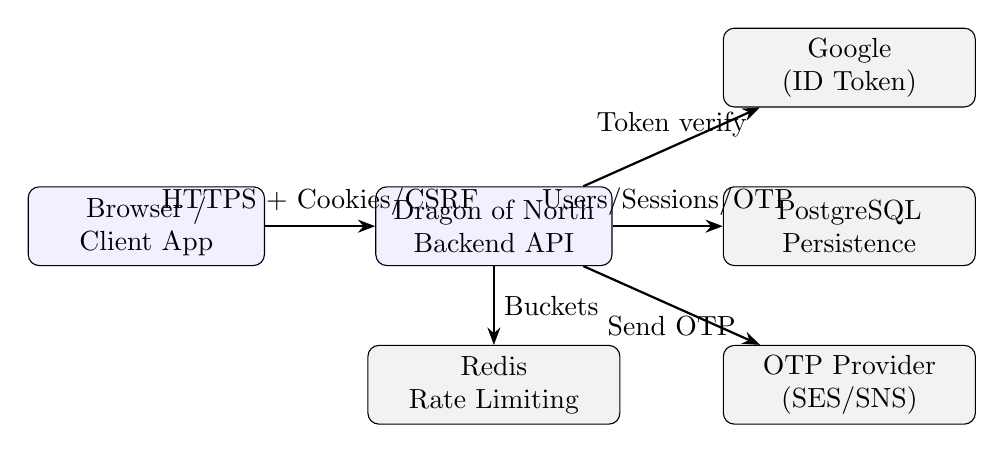
\begin{tikzpicture}[
            node distance=10mm and 14mm,
            box/.style={draw,rounded corners,align=center,minimum width=30mm,minimum height=10mm},
            ext/.style={draw,rounded corners,align=center,minimum width=32mm,minimum height=10mm,fill=gray!10},
            arrow/.style={-{Stealth[length=2.2mm]},thick}
        ]
            \node[box,fill=blue!6] (client) {Browser /\\Client App};
            \node[box,fill=blue!6,right=of client] (api) {\ProductName{}\\Backend API};
            \node[ext,above right=of api] (google) {Google\\(ID Token)};
            \node[ext,below right=of api] (aws) {OTP Provider\\(SES/SNS)};
            \node[ext,below=of api] (redis) {Redis\\Rate Limiting};
            \node[ext,right=of api] (pg) {PostgreSQL\\Persistence};

            \draw[arrow] (client) -- node[above]{HTTPS + Cookies/CSRF} (api);
            \draw[arrow] (api) -- node[above]{Token verify} (google);
            \draw[arrow] (api) -- node[below]{Send OTP} (aws);
            \draw[arrow] (api) -- node[right]{Buckets} (redis);
            \draw[arrow] (api) -- node[above]{Users/Sessions/OTP} (pg);
        \end{tikzpicture}
        \caption{System context and external dependencies.}
        \label{fig:context}
    \end{figure}

    \subsection{Authentication Flow (High Level)}
    \begin{figure}[H]
        \centering
        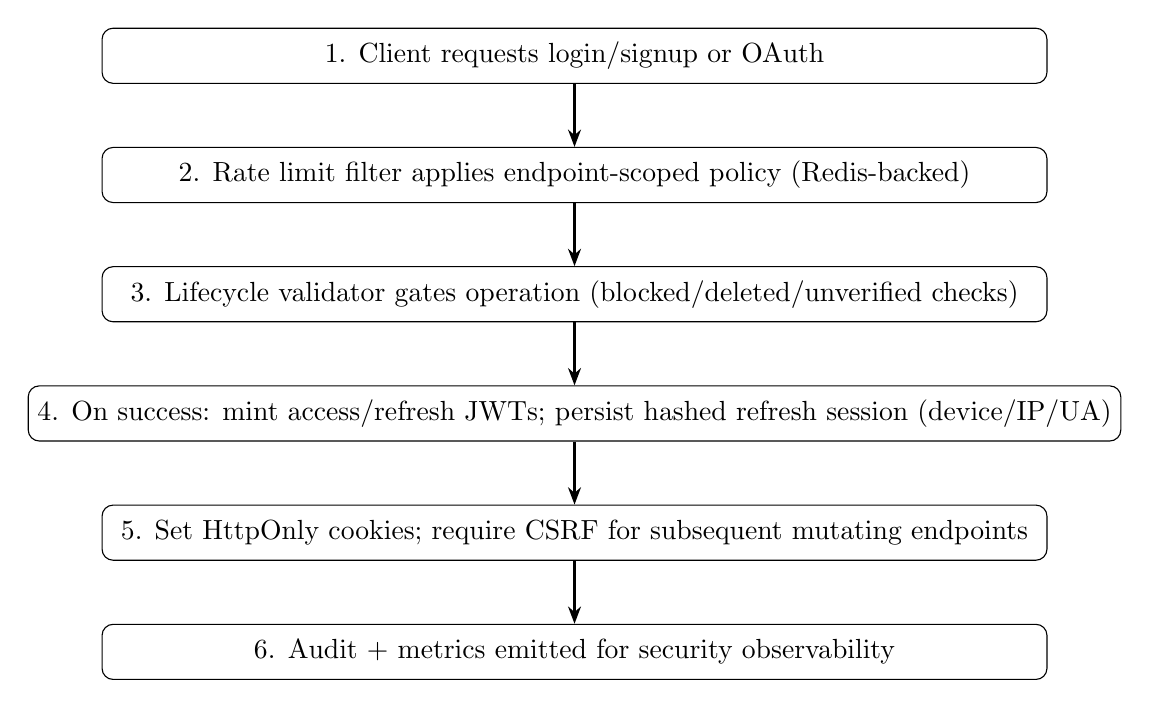
\begin{tikzpicture}[
            node distance=8mm,
            flowstep/.style={draw,rounded corners,align=left,minimum width=120mm,minimum height=7mm},
            arrow/.style={-{Stealth[length=2.2mm]},thick}
        ]
            \node[flowstep] (s1) {1. Client requests login/signup or OAuth};
            \node[flowstep,below=of s1] (s2) {2. Rate limit filter applies endpoint-scoped policy (Redis-backed)};
            \node[flowstep,below=of s2] (s3) {3. Lifecycle validator gates operation (blocked/deleted/unverified checks)};
            \node[flowstep,below=of s3] (s4) {4. On success: mint access/refresh JWTs; persist hashed refresh session (device/IP/UA)};
            \node[flowstep,below=of s4] (s5) {5. Set HttpOnly cookies; require CSRF for subsequent mutating endpoints};
            \node[flowstep,below=of s5] (s6) {6. Audit + metrics emitted for security observability};
            \draw[arrow] (s1) -- (s2);
            \draw[arrow] (s2) -- (s3);
            \draw[arrow] (s3) -- (s4);
            \draw[arrow] (s4) -- (s5);
            \draw[arrow] (s5) -- (s6);
        \end{tikzpicture}
        \caption{High-level authentication pipeline.}
        \label{fig:auth-flow}
    \end{figure}

    \subsection{Refresh Token Rotation (Sequence)}
    \begin{figure}[H]
        \centering
        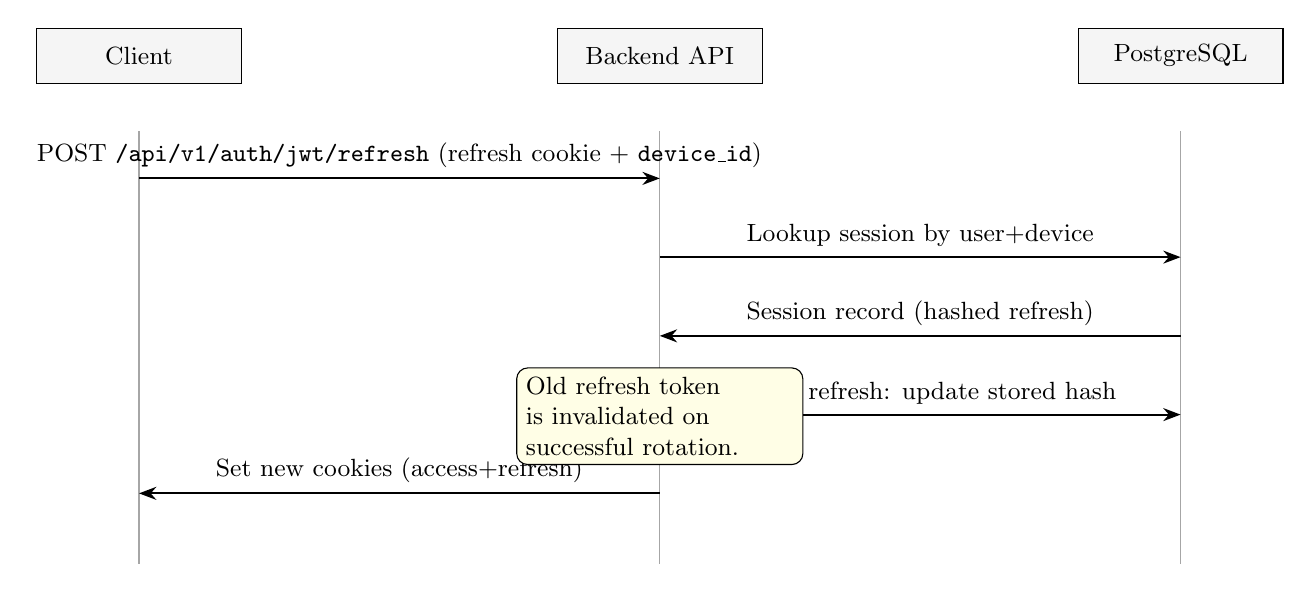
\begin{tikzpicture}[
            font=\small,
            lifeline/.style={draw,minimum width=26mm,minimum height=7mm,align=center,fill=gray!8},
            arrow/.style={-{Stealth[length=2.2mm]},thick},
            note/.style={draw,rounded corners,fill=yellow!10,align=left}
        ]
            \node[lifeline] (c) {Client};
            \node[lifeline, right=40mm of c] (a) {Backend API};
            \node[lifeline, right=40mm of a] (d) {PostgreSQL};

            \coordinate (c1) at ($(c.south)+(0,-6mm)$);
            \coordinate (a1) at ($(a.south)+(0,-6mm)$);
            \coordinate (d1) at ($(d.south)+(0,-6mm)$);

            \draw[gray!70] (c1) -- ++(0,-55mm);
            \draw[gray!70] (a1) -- ++(0,-55mm);
            \draw[gray!70] (d1) -- ++(0,-55mm);

            \draw[arrow] ($(c1)+(0,-6mm)$) -- node[above]{POST \texttt{/api/v1/auth/jwt/refresh} (refresh cookie + \texttt{device\_id})} ($(a1)+(0,-6mm)$);
            \draw[arrow] ($(a1)+(0,-16mm)$) -- node[above]{Lookup session by user+device} ($(d1)+(0,-16mm)$);
            \draw[arrow] ($(d1)+(0,-26mm)$) -- node[above]{Session record (hashed refresh)} ($(a1)+(0,-26mm)$);
            \draw[arrow] ($(a1)+(0,-36mm)$) -- node[above]{Rotate refresh: update stored hash} ($(d1)+(0,-36mm)$);
            \draw[arrow] ($(a1)+(0,-46mm)$) -- node[above]{Set new cookies (access+refresh)} ($(c1)+(0,-46mm)$);

            \node[note, anchor=north, text width=34mm, align=left] at ($(a1)+(0,-30mm)$) {Old refresh token\\is invalidated on\\successful rotation.};
        \end{tikzpicture}
        \caption{Sequence of refresh token rotation with session store validation.}
        \label{fig:refresh-seq}
    \end{figure}

% ---------------------------------------------------------------------------
    \appendix


    \section{Appendix A: API Endpoint Summary}
    \begin{table}[H]
        \centering
        \footnotesize
        \begin{tabularx}{\textwidth}{@{}l>{\raggedright\arraybackslash}X@{}}
    \toprule
    \textbf{Area} & \textbf{Representative Endpoints (non-exhaustive)} \\
    \midrule
    Identifier auth & \nolinkurl{/api/v1/auth/identifier/status}, \nolinkurl{/api/v1/auth/identifier/sign-up}, \nolinkurl{/api/v1/auth/identifier/sign-up/complete}, \nolinkurl{/api/v1/auth/identifier/login}, \nolinkurl{/api/v1/auth/identifier/logout} \\
    Token refresh & \nolinkurl{/api/v1/auth/jwt/refresh} \\
    CSRF bootstrap & \nolinkurl{/api/v1/auth/csrf} \\
    Password lifecycle & \nolinkurl{/api/v1/auth/password/forgot/request}, \nolinkurl{/api/v1/auth/password/forgot/reset}, \nolinkurl{/api/v1/auth/password/change} \\
    Account & \nolinkurl{/api/v1/auth/account/delete} \\
    OTP & \nolinkurl{/api/v1/otp/email/request}, \nolinkurl{/api/v1/otp/email/verify}, \nolinkurl{/api/v1/otp/phone/request}, \nolinkurl{/api/v1/otp/phone/verify} \\
    OAuth & \nolinkurl{/api/v1/auth/oauth/google}, \nolinkurl{/api/v1/auth/oauth/google/signup} \\
    Profile & \nolinkurl{/api/v1/profile} (GET/PATCH), \nolinkurl{/api/v1/profile/image} (multipart) \\
    Sessions & \nolinkurl{/api/v1/sessions/get/all}, \nolinkurl{/api/v1/sessions/delete/\{sessionId\}}, \nolinkurl{/api/v1/sessions/revoke-others} \\
    \bottomrule
        \end{tabularx}
        \caption{Endpoint summary for quick navigation.}
        \label{tab:endpoints}
    \end{table}


    \section{Appendix B: Data Entities (Conceptual)}
    \begin{itemize}
        \item \textbf{User}: identifier(s), credential metadata, lifecycle state, timestamps.
        \item \textbf{Auth Provider}: mapping of user to provider type (LOCAL/GOOGLE), constraints on login method.
        \item \textbf{Session}: device-scoped refresh session; hashed refresh token; IP/user-agent; revoked state.
        \item \textbf{OTP Token}: identifier + purpose + hashed OTP; TTL; attempts; consumed state.
        \item \textbf{Profile}: username/display name/bio/avatar URL; linked to user.
        \item \textbf{Roles/Permissions}: foundational tables for future RBAC expansion.
    \end{itemize}

\end{document}
